\documentclass[a4paper,11pt]{article}



% * Activating Greek fonts in Latex
  \usepackage[english,greek]{babel} % the last language is the default

  %% > UNCOMMENT if your editor uses iso-8859-7 encoding for Greek (typical in Windows System).
  \usepackage[iso-8859-7]{inputenc}

  %% > UNCOMMENT if your editor uses Unicode encoding for Greek (typical in POSIX Systems).
 % \usepackage[utf8x]{inputenc}


  \newcommand{\lt}{\latintext}
  \newcommand{\gt}{\greektext}


% * Math packages
 % \usepackage{amsthm}
  \usepackage{amsmath}
  \usepackage{array}
  \usepackage{multirow}
  \usepackage{enumitem}
  \usepackage{pgfplots}



 % \usepackage{amssymb}

% * graphics package
%  \usepackage[pdftex]{graphicx} % remove the 'pdftex' option if not PDFLatex is used.

% * verbatim writing package (mainly used to import program's code)
  \usepackage{verbatim}

% ------------------------------------------------------------------------------- %


% ------------------------------------------------------------------------------- %
% Here we set the title, the author and the date of our document.
%
% * Setting the title of the document
  \title{Πρώτη εργασία  - Αριθμητική Ανάλυση} % Put your own title here

% * Setting the author or authors of the document
  \author{Όνοματεπώνυμο: Θανάσης Ξανθόπουλος  \\  ΑΕΜ: 2392}       % Put your own Name and AEM here

% * Setting the date of the document
  \date{\today}                                      % Put a specific date here
% ------------------------------------------------------------------------------- %


% =============================================================================== %
% ||                       HERE WE BEGIN OUR DOCUMENT                          || %
% =============================================================================== %
\begin{document}



% Command that prints the title of your document
\maketitle
(Οι υλοποιήσεις των ασκήσεων έγιναν σε \lt\textbf{python 3} \gt και χρησιμοποιήθκαν οι βιβλιοθήκες \lt \textbf{math}, \lt \textbf{random}, \lt \textbf{matplotlib.pyplot}, \lt \textbf{datetime} \gt και \lt \textbf{numpy}) \gt
\section{Πρώτη ¶σκηση}
\subsection{Λύση}


    \begin{center}
    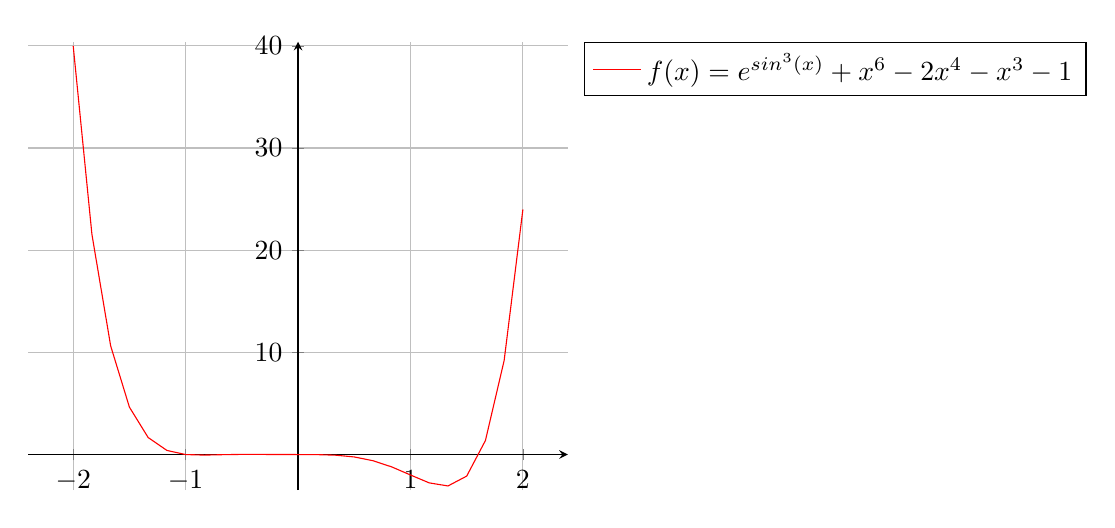
\begin{tikzpicture}
    \begin{axis}[grid=both,axis lines=middle,domain=-2:2,legend pos=outer north east,enlargelimits={abs=0.4},xticklabels={$-2$,$-1$, $0$,$1$,$2$},xtick={-2,-1,0,1,2}]
    \addplot[red] { exp(1) ^ ((sin(x)) ^ 3) + x ^ 6 - 2 * x ^ 4 - x ^ 3 - 1}; 
    \legend{$f(x)=e^{sin^3(x)} + x^6 - 2 x^4 - x^3 - 1$}
    \end{axis}
\end{tikzpicture}
	\end{center}
	
	\begin{flushleft}
Στο αρχείο \lt 
\begin{verbatim} askisi1_2392.py
 \end{verbatim} 
 \gt βρίσκονται οι υλοποιήσεις των μεθόδων που ζητήθηκαν καθώς και η εκτέλεση αυτών με δοκιμαστικές τιμές.\linebreak \\

\begin{itemize}
\item Η συνάρτηση \lt \textbf{bisection} \gt επιστρέφει το αποτέλεσμα της μεθόδου διχοτόμησης με την ακριβεια που ορίζουμε, πιο συγκεκριμένα:\linebreak 
\begin{enumerate}
\item πρωτο όρισμα \lt \textbf{f}: \gt Η συνάρτηση
\item δεύτερο όρισμα \lt \textbf{a}: \gt Το ένα από τα δύο άκρα
\item τρίτο ορισμα \lt \textbf{b}: \gt Το δεύτερο από τα δύο άκρα
\item τέταρτο όρισμα \lt \textbf{n}: \gt Η ακρίβεια δεκαδικού ψηφίου που θέλουμε
\end{enumerate}\pagebreak 
Ο τρόπος που λειτουργεί είναι ο εξής:\linebreak 
	Εφόσον η διαφορά των δύο σημείων είναι μεγαλύερη απο την ακρίβεια που έχουμε ορίσει, (αρχή διαδικασίας) τότε βρες το μέσο των δύο αυτών σημείων και έλεγξε για αρχή μήπως είναι ρίζα (άμα είναι σταμάτα την διαδικασία και επέστρεψε το αποτέλεσμα). Έλεγξε τις συνθήκες \lt bolzano \gt για τα σημεία \lt m\gt (μέσο) και \lt a, \gt άν ισχύουν τότε θέσε στη μεταβλητή του άλλου σημείου \lt b \gt την τιμή του \lt m\gt (μέσο), αλλιώς θέσε στη μεταβλητή σημείου \lt a \gt την τιμή του \lt m\gt (μέσο) και επανέλαβε την διαδικασία.\linebreak \\
	
	
\item Η συνάρτηση \lt \textbf{newtonraphson} \gt επιστρέφει το αποτέλεσμα της μεθόδου \lt Newton-Raphson \gt με την ακριβεια που ορίζουμε, πιο συγκεκριμένα:\linebreak 
	\begin{enumerate}
\item πρωτο όρισμα \lt \textbf{f}: \gt Η συνάρτηση
\item δεύτερο όρισμα \lt \textbf{f\_par}: \gt Η παράγωγος της συνάρτησης \lt \textbf{f} 
\item \gt τρίτο όρισμα \lt \textbf{x0}: \gt Σημείο που επιλέγουμε (πρεπει να ικανοποιεί την συνθήκη \lt $f(x0)*f''(x0)>0$
\item \gt τέταρτο όρισμα \lt \textbf{n}: \gt Η ακρίβεια δεκαδικού ψηφίου που θέλουμε
\end{enumerate}
Ο τρόπος που λειτουργεί είναι ο εξής:\linebreak 
	Αρχικά έλεγξε άμα ικανοποιείται η συνηνθήκη $f(x0)f''(x0)>0$\linebreak
	Έπειτε θέσε στην μεταβλητη $x$ την τιμή του $x0$ (για λόγους αναγνωσιμώτητας του κώδικα), και στην μεταβλητή $h$ την τιμή $\frac{f(x)}{f'(x)}$.
	Όσο η τιμή της μεταβλητής $h$ είναι μεγαλύερη ή ίση με τον αριθμό που έχουμε θέσει ως ακρίβεια ($n$ δεκαδικά ψηφία, όπου ακρίβεια: $10^{-n}$), έλεγξε άν το $x$ είναι ρίζα, άμα είναι βγες από τον βρόγχο και επέστρεψε την αποτέλεσμα(τέλος),\linebreak
	έπειτα, (αρχή διαδικασίας) θέσε στην μεταβλητή $h$ την τιμή $\frac{f(x)}{f'(x)}$ και στην μεταβλητή $x$ την τιμή $x-h$ και επανέλαβε την διαδικασία.  
	\linebreak
	
	\item Η συνάρτηση \lt \textbf{temnousa} \gt επιστρέφει το αποτέλεσμα της μεθόδου της Τέμνουσας με την ακριβεια που ορίζουμε, πιο συγκεκριμένα:\linebreak 
	\begin{enumerate}
\item πρωτο όρισμα \lt \textbf{f}: \gt Η συνάρτηση
\item δεύτερο όρισμα \lt \textbf{x0}: \gt Το πρώτο από τα δύο σημεία 
\item \gt τρίτο όρισμα \lt \textbf{x1}: \gt Το δεύτερο απο τα δύο σημεία
\item \gt τέταρτο όρισμα \lt \textbf{n}: \gt Η ακρίβεια δεκαδικού ψηφίου που θέλουμε
\end{enumerate}\pagebreak 
Ο τρόπος που λειτουργεί είναι ο εξής:\linebreak 
	Όσο η απόλυτη τιμή της διαφοράς $f(x1)-f(x0)$ είναι μεγαλύτερη ή ίση με την τιμή του σφάλματος, έλεγξε άν το σημείο $x0$ είναι ρίζα της συνάρτησης, άμα είναι βγες από τον βρόγχο και επέστρεψε την αποτέλεσμα(τέλος),\linebreak
	έπειτα, θέσε στην μεταβλητή $x\_temp$ την τιμή $x1 - \frac{f(x1)(x1-x0)}{f(x1)-f(x0)}$, την μεταβλητή $x0$ την τιμή της μεταβλητής $x1$ και στην μεταβλητή $x1$ την τιμή της μεταββλητής $x\_temp$, επανέλαβε την διαδικασία μέχρι να ικανοποιηθεί η συνθήκη (η απόλυτη τιμή της διαφοράς $f(x1)-f(x0)$ είναι μεγαλύτερη ή ίση με την τιμή του σφάλματος).
	\subsection{Αποτελέσματα}
\medskip 
---\emph{\textbf{Μέθοδος Διχοτόμησης}}---\\
Τιμές: $(-2, 1.5)$\quad   Προσσέγγιση ρίζας: $-1.19763$\quad Επαναλήψεις: 18\\
Τιμές: $(0, 2)$\quad Προσσέγγιση ρίζας: $1.53013$\quad Επαναλήψεις: 17\\
Τιμές: $(-2, 2)$\quad Προσσέγγιση ρίζας: $0.00000$\quad Επαναλήψεις: 1\\
\bigskip 
---\emph{\textbf{Μέθοδος \lt Newton Raphson\gt}}---\\
Τιμή: $(-2)$\quad      Προσσέγγιση ρίζας: $-1.19762$\quad 	Επαναλήψεις: 8\\
Τιμή: $(2)$\quad	  Προσσέγγιση ρίζας: $1.53013$\quad 	Επαναλήψεις: 6\\
Τιμή: $(0.5)$\quad	  Προσσέγγιση ρίζας: $0.00009$\quad 	Επαναλήψεις: 30\\
\bigskip 
---\emph{\textbf{Μέθοδος Τέμνουσας}}---\\
Τιμές: $(-2, 0)$\quad		 Προσσέγγιση ρίζας: $0.00000$\quad 	Επαναλήψεις: 1\\
Τιμές: $(-2, -1)$\quad		 Προσσέγγιση ρίζας: $-1.19762$\quad 	Επαναλήψεις: 14\\
Τιμές: $(-2, 2)$\quad		 Προσσέγγιση ρίζας: $1.53013$\quad 	Επαναλήψεις: 12\\

	\end{itemize}
	\end{flushleft}

\pagebreak


\section{Δεύτερη ¶σκηση}
\subsection{Λύση}
\begin{flushleft}
Στο αρχείο \lt 
\begin{verbatim} askisi1_2392.py
 \end{verbatim} 
 \gt βρίσκονται οι υλοποιήσεις των τροποποιημένων μεθόδων που ζητήθηκαν καθώς και η εκτέλεση αυτών με δοκιμαστικές τιμές.\linebreak \\

\item Η συνάρτηση \lt \textbf{newtonraphson\_mod} \gt επιστρέφει το αποτέλεσμα της τροποποιημένης μεθόδου \lt Newton-Raphson \gt με την ακριβεια που ορίζουμε, πιο συγκεκριμένα:\linebreak 
	\begin{enumerate}
\item πρωτο όρισμα \lt \textbf{f}: \gt Η συνάρτηση
\item δεύτερο όρισμα \lt \textbf{f\_par1}: \gt Η πρώτη παράγωγος της συνάρτησης \lt \textbf{f} 
\item\gt τρίτο όρισμα \lt \textbf{f\_par2}: \gt Η δεύτερη παράγωγος της συνάρτησης \lt \textbf{f}
\item \gt τρίτο όρισμα \lt \textbf{x0}: \gt Σημείο που επιλέγουμε (πρεπει να ικανοποιεί την συνθήκη \lt $f(x0)*f''(x0)>0$
\item \gt τέταρτο όρισμα \lt \textbf{n}: \gt Η ακρίβεια δεκαδικού ψηφίου που θέλουμε
\end{enumerate}
Ο τρόπος που λειτουργεί είναι ο εξής:\linebreak 
	Αρχικά έλεγξε άμα ικανοποιείται η συνηνθήκη $f(x0)f''(x0)>0$\linebreak
	Έπειτε θέσε στην μεταβλητη $x$ την τιμή του $x0$ (για λόγους αναγνωσιμώτητας του κώδικα) και στην μεταβλητή $h$ την τιμή $\frac{1}{\frac{f'(x)}{f(x)}-\frac{1}{2}\frac{f''(x)}{f'(x)}}$.
	Όσο η τιμή της μεταβλητής $h$ είναι μεγαλύερη ή ίση με τον αριθμό που έχουμε θέσει ως ακρίβεια ($n$ δεκαδικά ψηφία, όπου ακρίβεια: $10^{-n}$), έλεγξε άν το $x$ είναι ρίζα, άμα είναι βγες από τον βρόγχο και επέστρεψε την αποτέλεσμα(τέλος),\linebreak
	έπειτα, (αρχή διαδικασίας) θέσε στην μεταβλητή $h$ την τιμή $\frac{1}{\frac{f'(x)}{f(x)}-\frac{1}{2}\frac{f''(x)}{f'(x)}}$ και στην μεταβλητή $x$ την τιμή $x-h$ και επανέλαβε την διαδικασία.  
	\linebreak


\begin{itemize}
\item Η συνάρτηση \lt \textbf{bisection\_mod} \gt επιστρέφει το αποτέλεσμα της τροποποιημένης μεθόδου διχοτόμησης με την ακριβεια που ορίζουμε, πιο συγκεκριμένα:\linebreak 
\begin{enumerate}
\item πρωτο όρισμα \lt \textbf{f}: \gt Η συνάρτηση
\item δεύτερο όρισμα \lt \textbf{a}: \gt Το ένα από τα δύο άκρα
\item τρίτο ορισμα \lt \textbf{b}: \gt Το δεύτερο από τα δύο άκρα
\item τέταρτο όρισμα \lt \textbf{n}: \gt Η ακρίβεια δεκαδικού ψηφίου που θέλουμε
\end{enumerate}
Ο τρόπος που λειτουργεί είναι ο εξής:\linebreak 
	Εφόσον η διαφορά των δύο σημείων είναι μεγαλύερη απο την ακρίβεια που έχουμε ορίσει, (αρχή διαδικασίας) τότε βρες το μέσο των δύο αυτών σημείων και έλεγξε για αρχή μήπως είναι ρίζα (άμα είναι σταμάτα την διαδικασία και επέστρεψε το αποτέλεσμα). Έλεγξε τις συνθήκες \lt bolzano \gt για τα σημεία \lt r\gt (μέσο) και \lt a, \gt άν ισχύουν τότε θέσε στη μεταβλητή του άλλου σημείου \lt b \gt την τιμή του \lt r\gt (τυχαίο σημείο μεταξύ \lt (a, b))\gt, αλλιώς θέσε στη μεταβλητή σημείου \lt a \gt την τιμή του \lt r\gt (τυχαίο σημείο μεταξύ \lt (a, b))\gt και επανέλαβε την διαδικασία.\gt\linebreak \\
	
	

	
	\item Η συνάρτηση \lt \textbf{temnousa\_mod} \gt επιστρέφει το αποτέλεσμα της τροποποιημένης μεθόδου της Τέμνουσας με την ακριβεια που ορίζουμε, πιο συγκεκριμένα:\linebreak 
	\begin{enumerate}
\item πρωτο όρισμα \lt \textbf{f}: \gt Η συνάρτηση
\item δεύτερο όρισμα \lt \textbf{x0}: \gt Το πρώτο από τα τρία σημεία 
\item \gt τρίτο όρισμα \lt \textbf{x1}: \gt Το δεύτερο απο τα τρία σημεία
\item \gt τέταρτο όρισμα \lt \textbf{x2}: \gt Το τρίτο απο τα τρία σημεία
\item \gt πέμπτο όρισμα \lt \textbf{n}: \gt Η ακρίβεια δεκαδικού ψηφίου που θέλουμε
\end{enumerate}
Ο τρόπος που λειτουργεί είναι ο εξής:\linebreak 
	Όσο η απόλυτη τιμή της διαφοράς $f(x1)-f(x0)$ είναι μεγαλύτερη ή ίση με την τιμή του σφάλματος (αρχή διαδικασίας), έλεγξε άν το σημείο $x0$ είναι ρίζα της συνάρτησης, άμα είναι βγες από τον βρόγχο και επέστρεψε την αποτέλεσμα(τέλος),\linebreak
	έπειτα, θέσε στην μεταβλητή $x\_temp$ την τιμή $x2 - \frac{r(r-q)(x2-x1)+(1-r)s(x2-x0)}{(q-1)(r-1)(s-1)}$, την μεταβλητή $x0$ την τιμή της μεταβλητής $x1$, την μεταβλητή $x1$ την τιμή της μεταββλητής $x2$ και στην μεταβλητή $x2$ την τιμή της μεταβλητής $x\_temp$, επανέλαβε την διαδικασία μέχρι να ικανοποιηθεί η συνθήκη (η απόλυτη τιμή της διαφοράς $f(x1)-f(x0)$ είναι μεγαλύτερη ή ίση με την τιμή του σφάλματος). *Όπου $q$, $r$, $s$ : $q=\frac{f(x0)}{f(x1)}$, $r=\frac{f(x2)}{f(x1)}$, $s=\frac{f(x2)}{f(x0)}$.
	\pagebreak
	\subsection{Αποτελέσματα}
\medskip 

---\emph{\textbf{Τροποποιημένη Μέθοδος \lt Newton Raphson\gt}}---\\
Τιμή: $(-2)$\quad      Προσσέγγιση ρίζας: $-1.38130$\quad 	Επαναλήψεις: 5\\
Τιμή: $(-1)$\quad	  Προσσέγγιση ρίζας: $-0.66667$\quad 	Επαναλήψεις: 11\\
Τιμή: $(3/4)$\quad	  Προσσέγγιση ρίζας: $0.50000$\quad 	Επαναλήψεις: 4\\
Τιμή: $(1.5)$\quad	  Προσσέγγιση ρίζας: $1.17612$\quad 	Επαναλήψεις: 4\\
Τιμή: $(3/20)$\quad	  Προσσέγγιση ρίζας: $0.20518$\quad 	Επαναλήψεις: 3\\
\bigskip 

---\emph{\textbf{Τροποποιημένη Μέθοδος Διχοτόμησης}}---\\
Τιμές: $(-2, -1)$\quad Προσσέγγιση ρίζας: $-1.38130$\quad Επαναλήψεις: 22\\
Τιμές: $(-1, 0.5)$\quad Προσσέγγιση ρίζας: $0.20519$\quad Επαναλήψεις: 29\\
Τιμές: $(1, 2)$\quad Προσσέγγιση ρίζας: $1.17612$\quad Επαναλήψεις: 15\\
Τιμές: $(0.3, 1)$\quad Προσσέγγιση ρίζας: $0.50000$\quad Επαναλήψεις: 18\\
Τιμές: $(-0.69, -0.66)$\quad Προσσέγγιση ρίζας: $-0.66000$\quad Επαναλήψεις: 9\\
\bigskip 

---\emph{\textbf{Τροποποιημένη Μέθοδος Τέμνουσας}}---\\
Τιμές: $(-2, 0, 2)$\quad Προσσέγγιση ρίζας: $0.20518$\quad 	Επαναλήψεις: 8\\
Τιμές: $(0, 1, 2)$\quad Προσσέγγιση ρίζας: $-0.66645$\quad 	Επαναλήψεις: 14\\
Τιμές: $(1, 0, 1.5)$\quad Προσσέγγιση ρίζας: $0.50000$\quad 	Επαναλήψεις: 9\\
Τιμές: $(2, 1, 1.5)$\quad Προσσέγγιση ρίζας: $1.17612$\quad 	Επαναλήψεις: 11\\
Τιμές: $(-1, -1.5, -1.4)$\quad Προσσέγγιση ρίζας: $-1.38130$\quad 	Επαναλήψεις: 7\\

	\end{itemize}
	\end{flushleft}


% =============================================================================== %
% ||                       HERE WE END OUR DOCUMENT                          || %
% =============================================================================== %
\end{document}
